\documentclass[12pt,a4paper]{article}

\usepackage[utf8]{inputenc}
\usepackage[T2A]{fontenc}
\usepackage[ukrainian]{babel}

\usepackage{geometry}
\geometry{left=2cm,right=2cm,top=2cm,bottom=2cm}

\usepackage{graphicx}
\usepackage{array,multirow}
\usepackage{booktabs}
\usepackage{caption}

\usepackage{subcaption}

\usepackage{tcolorbox}

\renewcommand{\thetable}{№\arabic{table}}
\captionsetup[table]{name=Таблиця}

\usepackage{amsmath}
\usepackage{pdflscape}
\usepackage{xcolor}

\usepackage{fvextra}
\usepackage{upquote}

\usepackage{hyperref}

\captionsetup[subfigure]{labelformat=simple,labelsep=space}

\usepackage{minted}

\usemintedstyle{vs}
\setminted{linenos, breaklines, frame=single, fontsize=\small}

\RecustomVerbatimCommand{\VerbatimInput}{VerbatimInput}{
    breaklines=true,
    breaksymbolleft={}
}

% Узагальнений стиль для коду
\newminted{java}{
  fontsize=\small,
  baselinestretch=1.05,
  breaklines,
  linenos,
  frame=lines,
  framesep=2mm
}

% Консоль/PowerShell як plain text
\newminted{text}{
  fontsize=\small,
  breaklines,
  frame=single,
  bgcolor=gray!5
}

\begin{document}

    \begin{titlepage}

        % Картинка шапки (по центру, з відступом від верху)
        \begin{center}
\includegraphics[width=0.7\textwidth]{../../../TITLES/letterhead.png}\end{center}

        \begin{center}
            \large Національний технічний університет України\\
            «Київський політехнічний інститут імені Ігоря Сікорського»\\[1em]
            Факультет інформатики та обчислювальної техніки\\
            Кафедра обчислювальної техніки
        \end{center}

        \vfill

        \begin{center}
            \textbf{\LARGE Інженерія програмного забезпечення}\\[2em]
            \textbf{\Large Практична робота №4}\\[0.5em]
            «Шаблони поведінки. Iterator, Mediator, Observer, Strategy, Chain of Responsibility»
        \end{center}

        \vfill

        \begin{flushright}
            Виконав: студент 2 курсу ФІОТ, гр. ІО-41\\
            \textit{Давидчук А.~М.}\\
            Залікова книжка № 4106\\[1em]
            Перевірив: \textit{Васильєва М.~Д.}
        \end{flushright}

        \vfill

        \begin{center}Київ --- 2025\end{center}

    \end{titlepage}

    % Основний документ:

    \setlength{\parindent}{0em}

    \textbf{\underline{Тема:}} «Шаблони поведінки. Iterator, Mediator, Observer, Strategy, Chain of Responsibility».

    \vspace{1em}

    \textbf{\underline{Мета:}} Ознайомлення з видами шаблонів проектування ПЗ. Вивчення шаблонів
    поведінки. Отримання базових навичок з застосування шаблонів Iterator, Mediator, Observer,
    Chain of Responsibility.

    \begin{center} \textbf{\Large Практична частина (Завдання №1)} \end{center}

    \setlength{\parindent}{1.5em}

    Мій номер залікової книги: $4106$, звідси $4106 \text{ mod } 13 = 11$. Тому умова до 1 завдання буде:

    Необхідно розробити класи, які моделюють основні елементи графічного інтерфейсу користувача (GUI), такі як вікна, кнопки та текстові області. Система повинна підтримувати реакцію на події, що виникають у будь-якому з елементів (натискання кнопки, зміна тексту, закриття вікна). GUI-елементи виступають як \textbf{джерела подій}, а \textbf{обробники подій (Listeners)} підписуються на сповіщення про них.

    \subsection*{Вимоги}

    \begin{itemize}
    \item \textbf{Базовий клас GUI-елемента (\texttt{GuiElement}):}
    \begin{itemize}
        \item містить загальні властивості:
        \begin{itemize}
        \item \texttt{id} — унікальний ідентифікатор;
        \item \texttt{name} — назва елемента;
        \item \texttt{visible} — стан видимості;
        \end{itemize}
        \item надає методи для:
        \begin{itemize}
        \item відображення / приховування елемента;
        \item керування списком слухачів подій (\texttt{addListener()}, \texttt{removeListener()}).
        \end{itemize}
    \end{itemize}

    \item \textbf{Інтерфейс обробника подій (\texttt{EventListener}):}
    \begin{itemize}
        \item містить метод \texttt{handleEvent(String eventType, GuiElement source)}, який викликається при виникненні подій.
    \end{itemize}

    \item \textbf{Класи конкретних GUI-елементів:}
    \begin{itemize}
        \item \textbf{Button:}
        \begin{itemize}
        \item має метод \texttt{click()}, який створює подію типу \texttt{"click"} і сповіщає всіх слухачів;
        \end{itemize}
        \item \textbf{TextField:}
        \begin{itemize}
        \item зберігає текст;
        \item має метод \texttt{setText(String text)}, який викликає подію \texttt{"textChanged"};
        \end{itemize}
        \item \textbf{Window:}
        \begin{itemize}
        \item зберігає заголовок і список вкладених елементів;
        \item може викликати подію типу \texttt{"close"}.
        \end{itemize}
    \end{itemize}

    \item \textbf{Слухачі подій} (наприклад, \texttt{Logger}, \texttt{ActionHandler}):
    \begin{itemize}
        \item реагують на події певного типу;
        \item можуть, наприклад, виводити повідомлення в консоль, змінювати інші елементи або виконувати певну дію.
    \end{itemize}

    \item \textbf{Забезпечити слабку зв’язність:} GUI-елементи не повинні напряму знати, що роблять слухачі — лише повідомляти про подію.
    \end{itemize}

    \subsection*{У методі \texttt{main} продемонструвати:}
    \begin{itemize}
    \item створення кількох GUI-елементів (вікно, кнопка, текстове поле);
    \item створення слухачів подій;
    \item підписку слухачів на події елементів;
    \item виклик кількох подій (натискання кнопки, зміна тексту);
    \item автоматичну реакцію слухачів на ці події.
    \end{itemize}

    \setlength{\parindent}{0em}

    \textbf{\underline{Загальна структура проекту до компіляції:}}

    \begin{minted}{text}
PS C:\Users\artem\Desktop\reps\university_roadmap\semestr3\software engineering\labs\lab4\project> tree /f /a
Folder PATH listing
Volume serial number is 1A5B-F8AF
C:.
|   build.xml
|
\---src
    \---work4
        |   DemoGuiSwing.java
        |
        \---gui
                ActionHandler.java
                Button.java
                EventListener.java
                GuiElement.java
                LoggerListener.java
                TextField.java
                Window.java
    \end{minted}

    \textbf{\underline{Код build.xml задля автоматизації:}}

    \begin{minted}{xml}
<?xml version="1.0" encoding="UTF-8"?>
<project name="work4-gui" default="dist" basedir=".">
    <!-- ==============================
         НАЛАШТУВАННЯ ПРОЄКТУ
         ============================== -->
    <property name="src.dir"       value="src"/>
    <property name="build.dir"     value="build"/>
    <property name="classes.dir"   value="${build.dir}/classes"/>
    <property name="dist.dir"      value="dist"/>
    <property name="docs.dir"      value="docs"/>
    <property name="jar.name"      value="work4-gui-demo.jar"/>

    <!-- Головний клас за замовчуванням (можна перевизначити: -Dmain.class=...) -->
    <property name="main.class"    value="work4.DemoGuiSwing"/>

    <!-- Налаштування компіляції Java -->
    <property name="javac.release" value="17"/>
    <property name="file.encoding" value="UTF-8"/>

    <!-- Клас-путь (додай зовнішні JAR, якщо потрібно) -->
    <path id="compile.classpath">
    </path>

    <!-- ==============================
         ЦІЛІ ЗБІРКИ
         ============================== -->

    <!-- Підказка по доступних цілях -->
    <target name="help" description="Show available build tasks">
        <echo>
Available Ant targets:
  ant clean                   - remove build, dist and docs directories
  ant compile                 - compile Java sources into build/classes
  ant run                     - run the main class (${main.class})
  ant jar                     - package compiled classes into dist/${jar.name}
  ant javadoc                 - generate documentation into docs/
  ant dist                    - full build: clean + compile + jar + javadoc

Override main class (example):
  ant -Dmain.class=work4.DemoGui run
        </echo>
    </target>

    <!-- Очистити результати попередніх збірок -->
    <target name="clean" description="Remove all generated files">
        <delete dir="${build.dir}"/>
        <delete dir="${dist.dir}"/>
        <delete dir="${docs.dir}"/>
    </target>

    <!-- Створити службові каталоги -->
    <target name="init">
        <mkdir dir="${classes.dir}"/>
        <mkdir dir="${dist.dir}"/>
        <mkdir dir="${docs.dir}"/>
    </target>

    <!-- Компіляція (через 'release' для узгоджених платформних модулів) -->
    <target name="compile" depends="init" description="Compile Java sources">
        <javac srcdir="${src.dir}"
               destdir="${classes.dir}"
               includeantruntime="false"
               release="${javac.release}"
               encoding="${file.encoding}"
               debug="true">
            <classpath refid="compile.classpath"/>
        </javac>
        <echo>Compilation completed successfully.</echo>
    </target>

    <!-- Запуск застосунку (можна перевизначити main.class через -D) -->
    <target name="run" depends="compile" description="Run the main class">
        <java classname="${main.class}" fork="true" dir=".">
            <classpath>
                <pathelement path="${classes.dir}"/>
                <path refid="compile.classpath"/>
            </classpath>
            <!-- Коректний UTF-8 вивід у консолі Windows/Unix -->
            <jvmarg value="-Dfile.encoding=${file.encoding}"/>
            <jvmarg value="-Dsun.stdout.encoding=${file.encoding}"/>
            <jvmarg value="-Dsun.stderr.encoding=${file.encoding}"/>
        </java>
    </target>

    <!-- Створення виконуваного JAR із маніфестом -->
    <target name="jar" depends="compile" description="Package into an executable JAR file">
        <jar destfile="${dist.dir}/${jar.name}" basedir="${classes.dir}">
            <manifest>
                <attribute name="Main-Class" value="${main.class}"/>
                <attribute name="Created-By" value="Apache Ant build.xml"/>
                <attribute name="Built-By" value="${user.name}"/>
            </manifest>
        </jar>
        <echo>JAR file created: ${dist.dir}/${jar.name}</echo>
    </target>

    <!-- Генерація Javadoc -->
    <target name="javadoc" description="Generate API documentation (Javadoc)">
        <javadoc destdir="${docs.dir}"
                 sourcepath="${src.dir}"
                 packagenames="work4.*"
                 encoding="${file.encoding}"
                 docencoding="${file.encoding}"
                 charset="${file.encoding}"
                 author="true"
                 version="true"
                 use="true"
                 splitindex="true"
                 windowtitle="work4 GUI - Javadoc"
                 failonerror="false">
            <link href="https://docs.oracle.com/en/java/javase/17/docs/api/"/>
        </javadoc>
        <echo>Javadoc generated in: ${docs.dir}</echo>
    </target>

    <!-- Повна збірка -->
    <target name="dist" depends="clean,compile,jar,javadoc"
            description="Perform full build (clean, compile, jar, javadoc)">
        <echo>Distribution build completed successfully.</echo>
    </target>
</project>
    \end{minted}

    \textbf{\underline{Перевірка:}}

    \begin{minted}{text}
PS C:\Users\artem\Desktop\reps\university_roadmap\semestr3\software engineering\labs\lab4\project> ant -p 
Buildfile: C:\Users\artem\Desktop\reps\university_roadmap\semestr3\software engineering\labs\lab4\project\build.xml

Main targets:

 clean    Remove all generated files
 compile  Compile Java sources
 dist     Perform full build (clean, compile, jar, javadoc)
 help     Show available build tasks
 jar      Package into an executable JAR file
 javadoc  Generate API documentation (Javadoc)
 run      Run the main class
Default target: dist
    \end{minted}

    \textbf{\underline{Загальна структура проекту після компіляції:}}
    
    \begin{minted}{text}
PS C:\Users\artem\Desktop\reps\university_roadmap\semestr3\software engineering\labs\lab4\project> ant 
Buildfile: C:\Users\artem\Desktop\reps\university_roadmap\semestr3\software engineering\labs\lab4\project\build.xml

clean:

init:
    [mkdir] Created dir: C:\Users\artem\Desktop\reps\university_roadmap\semestr3\software engineering\labs\lab4\project\build\classes
    [mkdir] Created dir: C:\Users\artem\Desktop\reps\university_roadmap\semestr3\software engineering\labs\lab4\project\dist
    [mkdir] Created dir: C:\Users\artem\Desktop\reps\university_roadmap\semestr3\software engineering\labs\lab4\project\docs

compile:
    [javac] Compiling 8 source files to C:\Users\artem\Desktop\reps\university_roadmap\semestr3\software engineering\labs\lab4\project\build\classes
     [echo] Compilation completed successfully.

jar:
      [jar] Building jar: C:\Users\artem\Desktop\reps\university_roadmap\semestr3\software engineering\labs\lab4\project\dist\work4-gui-demo.jar
     [echo] JAR file created: dist/work4-gui-demo.jar

javadoc:
  [javadoc] Generating Javadoc
  [javadoc] Javadoc execution
  [javadoc] Loading source files for package work4...
  [javadoc] Loading source files for package work4.gui...
  [javadoc] Constructing Javadoc information...
  [javadoc] Building index for all the packages and classes...
  [javadoc] Standard Doclet version 21.0.9+7-LTS-338
  [javadoc] Building tree for all the packages and classes...
  [javadoc] C:\Users\artem\Desktop\reps\university_roadmap\semestr3\software engineering\labs\lab4\project\src\work4\gui\GuiElement.java:9: error: unknown tag: pattern
  [javadoc]  * @pattern Observer: Subject (Publisher)
  [javadoc]    ^
  [javadoc] C:\Users\artem\Desktop\reps\university_roadmap\semestr3\software engineering\labs\lab4\project\src\work4\gui\EventListener.java:5: error: unknown tag: pattern
  [javadoc]  * @pattern Observer: Observer (Subscriber)
  [javadoc]    ^
  [javadoc] Generating C:\Users\artem\Desktop\reps\university_roadmap\semestr3\software engineering\labs\lab4\project\docs\work4\gui\ActionHandler.html...
  [javadoc] Generating C:\Users\artem\Desktop\reps\university_roadmap\semestr3\software engineering\labs\lab4\project\docs\work4\gui\Button.html...
  [javadoc] C:\Users\artem\Desktop\reps\university_roadmap\semestr3\software engineering\labs\lab4\project\src\work4\gui\GuiElement.java:32: warning: no main description
  [javadoc]     /** @return ????????? ?????????? ????????????? ???????? */
  [javadoc]         ^
  [javadoc] C:\Users\artem\Desktop\reps\university_roadmap\semestr3\software engineering\labs\lab4\project\src\work4\gui\GuiElement.java:35: warning: no main description
  [javadoc]     /** @return ??????? ????? ???????? */
  [javadoc]         ^
  [javadoc] C:\Users\artem\Desktop\reps\university_roadmap\semestr3\software engineering\labs\lab4\project\src\work4\gui\GuiElement.java:48: warning: no main description
  [javadoc]     /** @return ?? ? ??????? ??????? */
  [javadoc]         ^
  [javadoc] Generating C:\Users\artem\Desktop\reps\university_roadmap\semestr3\software engineering\labs\lab4\project\docs\work4\DemoGuiSwing.html...
  [javadoc] C:\Users\artem\Desktop\reps\university_roadmap\semestr3\software engineering\labs\lab4\project\src\work4\DemoGuiSwing.java:21: warning: use of default constructor, which does not provide a comment
  [javadoc] public class DemoGuiSwing {
  [javadoc]        ^
  [javadoc] C:\Users\artem\Desktop\reps\university_roadmap\semestr3\software engineering\labs\lab4\project\src\work4\DemoGuiSwing.java:22: warning: no comment
  [javadoc]     public static void main(String[] args) {
  [javadoc]                        ^
  [javadoc] Generating C:\Users\artem\Desktop\reps\university_roadmap\semestr3\software engineering\labs\lab4\project\docs\work4\gui\EventListener.html...
  [javadoc] Generating C:\Users\artem\Desktop\reps\university_roadmap\semestr3\software engineering\labs\lab4\project\docs\work4\gui\GuiElement.html...
  [javadoc] Generating C:\Users\artem\Desktop\reps\university_roadmap\semestr3\software engineering\labs\lab4\project\docs\work4\gui\LoggerListener.html...
  [javadoc] Generating C:\Users\artem\Desktop\reps\university_roadmap\semestr3\software engineering\labs\lab4\project\docs\work4\gui\TextField.html...
  [javadoc] C:\Users\artem\Desktop\reps\university_roadmap\semestr3\software engineering\labs\lab4\project\src\work4\gui\TextField.java:20: warning: no main description
  [javadoc]     /** @return ??????? ???????? ?????? */
  [javadoc]         ^
  [javadoc] Generating C:\Users\artem\Desktop\reps\university_roadmap\semestr3\software engineering\labs\lab4\project\docs\work4\gui\Window.html...
  [javadoc] C:\Users\artem\Desktop\reps\university_roadmap\semestr3\software engineering\labs\lab4\project\src\work4\gui\Window.java:26: warning: no main description
  [javadoc]     /** @return ???????? ????????? ????? */
  [javadoc]         ^
  [javadoc] Generating C:\Users\artem\Desktop\reps\university_roadmap\semestr3\software engineering\labs\lab4\project\docs\work4\package-summary.html...
  [javadoc] Generating C:\Users\artem\Desktop\reps\university_roadmap\semestr3\software engineering\labs\lab4\project\docs\work4\package-tree.html...
  [javadoc] Generating C:\Users\artem\Desktop\reps\university_roadmap\semestr3\software engineering\labs\lab4\project\docs\work4\gui\package-summary.html...
  [javadoc] Generating C:\Users\artem\Desktop\reps\university_roadmap\semestr3\software engineering\labs\lab4\project\docs\work4\gui\package-tree.html...
  [javadoc] Generating C:\Users\artem\Desktop\reps\university_roadmap\semestr3\software engineering\labs\lab4\project\docs\work4\class-use\DemoGuiSwing.html...
  [javadoc] Generating C:\Users\artem\Desktop\reps\university_roadmap\semestr3\software engineering\labs\lab4\project\docs\work4\gui\class-use\ActionHandler.html...
  [javadoc] Generating C:\Users\artem\Desktop\reps\university_roadmap\semestr3\software engineering\labs\lab4\project\docs\work4\gui\class-use\Button.html...
  [javadoc] Generating C:\Users\artem\Desktop\reps\university_roadmap\semestr3\software engineering\labs\lab4\project\docs\work4\gui\class-use\EventListener.html...
  [javadoc] Generating C:\Users\artem\Desktop\reps\university_roadmap\semestr3\software engineering\labs\lab4\project\docs\work4\gui\class-use\GuiElement.html...
  [javadoc] Generating C:\Users\artem\Desktop\reps\university_roadmap\semestr3\software engineering\labs\lab4\project\docs\work4\gui\class-use\LoggerListener.html...
  [javadoc] Generating C:\Users\artem\Desktop\reps\university_roadmap\semestr3\software engineering\labs\lab4\project\docs\work4\gui\class-use\TextField.html...
  [javadoc] Generating C:\Users\artem\Desktop\reps\university_roadmap\semestr3\software engineering\labs\lab4\project\docs\work4\gui\class-use\Window.html...
  [javadoc] Generating C:\Users\artem\Desktop\reps\university_roadmap\semestr3\software engineering\labs\lab4\project\docs\work4\package-use.html...
  [javadoc] Generating C:\Users\artem\Desktop\reps\university_roadmap\semestr3\software engineering\labs\lab4\project\docs\work4\gui\package-use.html...
  [javadoc] Generating C:\Users\artem\Desktop\reps\university_roadmap\semestr3\software engineering\labs\lab4\project\docs\overview-tree.html...
  [javadoc] Generating C:\Users\artem\Desktop\reps\university_roadmap\semestr3\software engineering\labs\lab4\project\docs\index.html...
  [javadoc] Building index for all classes...
  [javadoc] Generating C:\Users\artem\Desktop\reps\university_roadmap\semestr3\software engineering\labs\lab4\project\docs\allclasses-index.html...
  [javadoc] Generating C:\Users\artem\Desktop\reps\university_roadmap\semestr3\software engineering\labs\lab4\project\docs\allpackages-index.html...
  [javadoc] Generating C:\Users\artem\Desktop\reps\university_roadmap\semestr3\software engineering\labs\lab4\project\docs\index-files\index-1.html...
  [javadoc] Generating C:\Users\artem\Desktop\reps\university_roadmap\semestr3\software engineering\labs\lab4\project\docs\index-files\index-2.html...
  [javadoc] Generating C:\Users\artem\Desktop\reps\university_roadmap\semestr3\software engineering\labs\lab4\project\docs\index-files\index-3.html...
  [javadoc] Generating C:\Users\artem\Desktop\reps\university_roadmap\semestr3\software engineering\labs\lab4\project\docs\index-files\index-4.html...
  [javadoc] Generating C:\Users\artem\Desktop\reps\university_roadmap\semestr3\software engineering\labs\lab4\project\docs\index-files\index-5.html...
  [javadoc] Generating C:\Users\artem\Desktop\reps\university_roadmap\semestr3\software engineering\labs\lab4\project\docs\index-files\index-6.html...
  [javadoc] Generating C:\Users\artem\Desktop\reps\university_roadmap\semestr3\software engineering\labs\lab4\project\docs\index-files\index-7.html...
  [javadoc] Generating C:\Users\artem\Desktop\reps\university_roadmap\semestr3\software engineering\labs\lab4\project\docs\index-files\index-8.html...
  [javadoc] Generating C:\Users\artem\Desktop\reps\university_roadmap\semestr3\software engineering\labs\lab4\project\docs\index-files\index-9.html...
  [javadoc] Generating C:\Users\artem\Desktop\reps\university_roadmap\semestr3\software engineering\labs\lab4\project\docs\index-files\index-10.html...
  [javadoc] Generating C:\Users\artem\Desktop\reps\university_roadmap\semestr3\software engineering\labs\lab4\project\docs\index-files\index-11.html...
  [javadoc] Generating C:\Users\artem\Desktop\reps\university_roadmap\semestr3\software engineering\labs\lab4\project\docs\index-files\index-12.html...
  [javadoc] Generating C:\Users\artem\Desktop\reps\university_roadmap\semestr3\software engineering\labs\lab4\project\docs\index-files\index-13.html...
  [javadoc] Generating C:\Users\artem\Desktop\reps\university_roadmap\semestr3\software engineering\labs\lab4\project\docs\index-files\index-14.html...
  [javadoc] Generating C:\Users\artem\Desktop\reps\university_roadmap\semestr3\software engineering\labs\lab4\project\docs\index-files\index-15.html...
  [javadoc] Generating C:\Users\artem\Desktop\reps\university_roadmap\semestr3\software engineering\labs\lab4\project\docs\search.html...
  [javadoc] Generating C:\Users\artem\Desktop\reps\university_roadmap\semestr3\software engineering\labs\lab4\project\docs\overview-summary.html...
  [javadoc] Generating C:\Users\artem\Desktop\reps\university_roadmap\semestr3\software engineering\labs\lab4\project\docs\help-doc.html...
  [javadoc] 2 errors
  [javadoc] 7 warnings
     [echo] Javadoc generated in: docs

dist:
     [echo] Distribution build completed successfully.

BUILD SUCCESSFUL
Total time: 3 seconds

PS C:\Users\artem\Desktop\reps\university_roadmap\semestr3\software engineering\labs\lab4\project> tree /f /a
Folder PATH listing
Volume serial number is 1A5B-F8AF
C:.
|   build.xml
|
+---build
|   \---classes
|       \---work4
|           |   DemoGuiSwing$1.class
|           |   DemoGuiSwing$2.class
|           |   DemoGuiSwing.class
|           |
|           \---gui
|                   ActionHandler.class
|                   Button.class
|                   EventListener.class
|                   GuiElement.class
|                   LoggerListener.class
|                   TextField.class
|                   Window.class
|
+---dist
|       work4-gui-demo.jar
|
+---docs
|   |   allclasses-index.html
|   |   allpackages-index.html
|   |   copy.svg
|   |   element-list
|   |   help-doc.html
|   |   index.html
|   |   link.svg
|   |   member-search-index.js
|   |   module-search-index.js
|   |   overview-summary.html
|   |   overview-tree.html
|   |   package-search-index.js
|   |   script.js
|   |   search-page.js
|   |   search.html
|   |   search.js
|   |   stylesheet.css
|   |   tag-search-index.js
|   |   type-search-index.js
|   |
|   +---index-files
|   |       index-1.html
|   |       index-10.html
|   |       index-11.html
|   |       index-12.html
|   |       index-13.html
|   |       index-14.html
|   |       index-15.html
|   |       index-2.html
|   |       index-3.html
|   |       index-4.html
|   |       index-5.html
|   |       index-6.html
|   |       index-7.html
|   |       index-8.html
|   |       index-9.html
|   |
|   +---legal
|   |       COPYRIGHT
|   |       jquery.md
|   |       jqueryUI.md
|   |       LICENSE
|   |
|   +---resources
|   |       glass.png
|   |       x.png
|   |
|   +---script-dir
|   |       jquery-3.7.1.min.js
|   |       jquery-ui.min.css
|   |       jquery-ui.min.js
|   |
|   \---work4
|       |   DemoGuiSwing.html
|       |   package-summary.html
|       |   package-tree.html
|       |   package-use.html
|       |
|       +---class-use
|       |       DemoGuiSwing.html
|       |
|       \---gui
|           |   ActionHandler.html
|           |   Button.html
|           |   EventListener.html
|           |   GuiElement.html
|           |   LoggerListener.html
|           |   package-summary.html
|           |   package-tree.html
|           |   package-use.html
|           |   TextField.html
|           |   Window.html
|           |
|           \---class-use
|                   ActionHandler.html
|                   Button.html
|                   EventListener.html
|                   GuiElement.html
|                   LoggerListener.html
|                   TextField.html
|                   Window.html
|
\---src
    \---work4
        |   DemoGuiSwing.java
        |
        \---gui
                ActionHandler.java
                Button.java
                EventListener.java
                GuiElement.java
                LoggerListener.java
                TextField.java
                Window.java
    \end{minted}

    \newpage

    \textbf{\underline{Скріншоти результат виконання (демонстрації програми):}}

    \begin{figure}[h!]
        \centering

        \begin{subfigure}{1.0\textwidth}
            \centering
            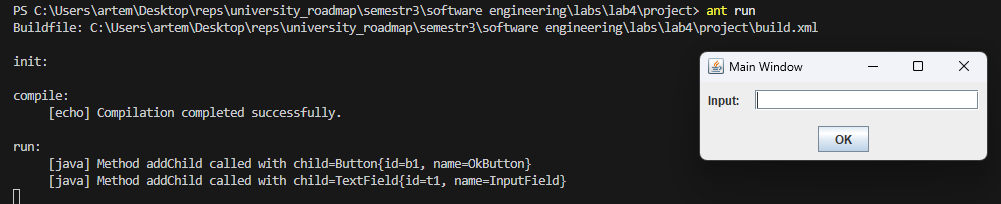
\includegraphics[width=\linewidth]{1-0.png}
        \end{subfigure}\vfill
        \begin{subfigure}{1.0\textwidth}
            \centering
            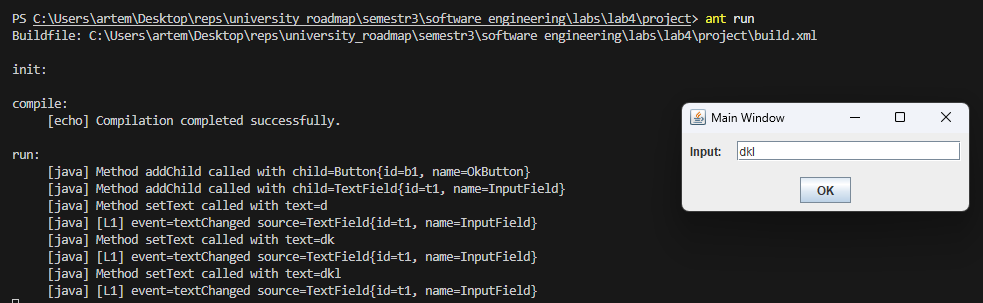
\includegraphics[width=\linewidth]{1-1.png}
        \end{subfigure}\vfill
        \begin{subfigure}{1.0\textwidth}
            \centering
            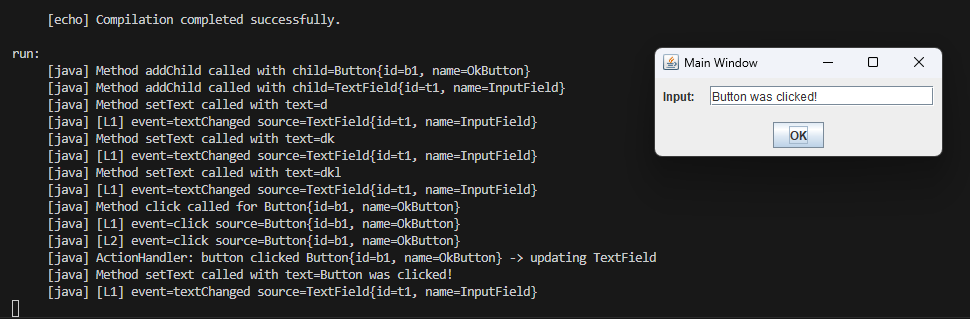
\includegraphics[width=\linewidth]{1-2.png}
        \end{subfigure}\vfill
        \begin{subfigure}{1.0\textwidth}
            \centering
            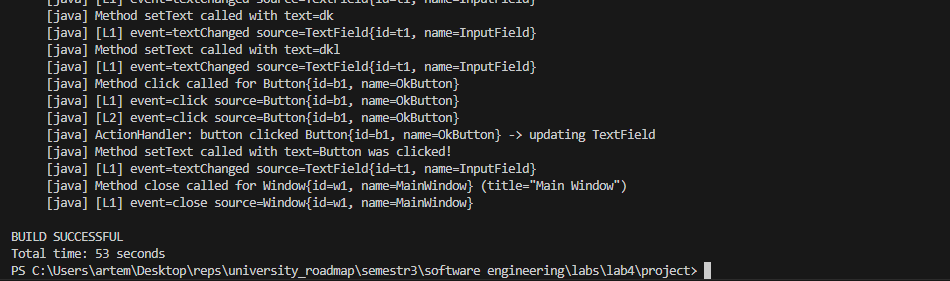
\includegraphics[width=\linewidth]{1-3.png}
        \end{subfigure}

    \end{figure}

    \newpage

    \textbf{\underline{Скріншот наявності документації:}}

    \begin{figure}[h!]
        \centering

        \begin{subfigure}{1.0\textwidth}
            \centering
            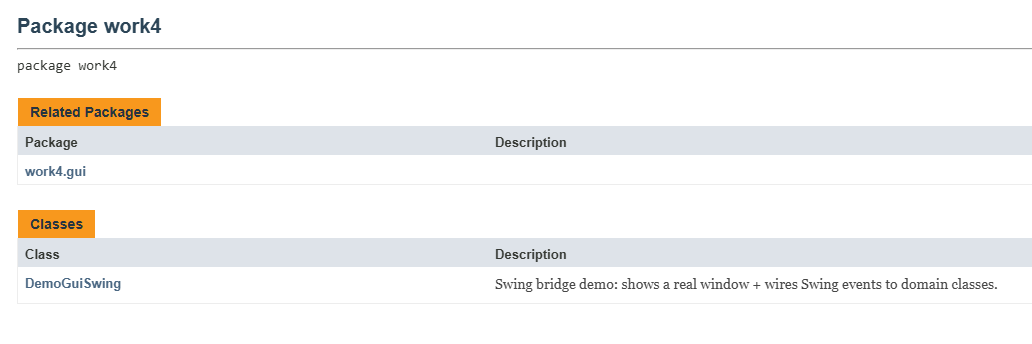
\includegraphics[width=\linewidth]{1-4.png}
        \end{subfigure}\vfill
        \begin{subfigure}{1.0\textwidth}
            \centering
            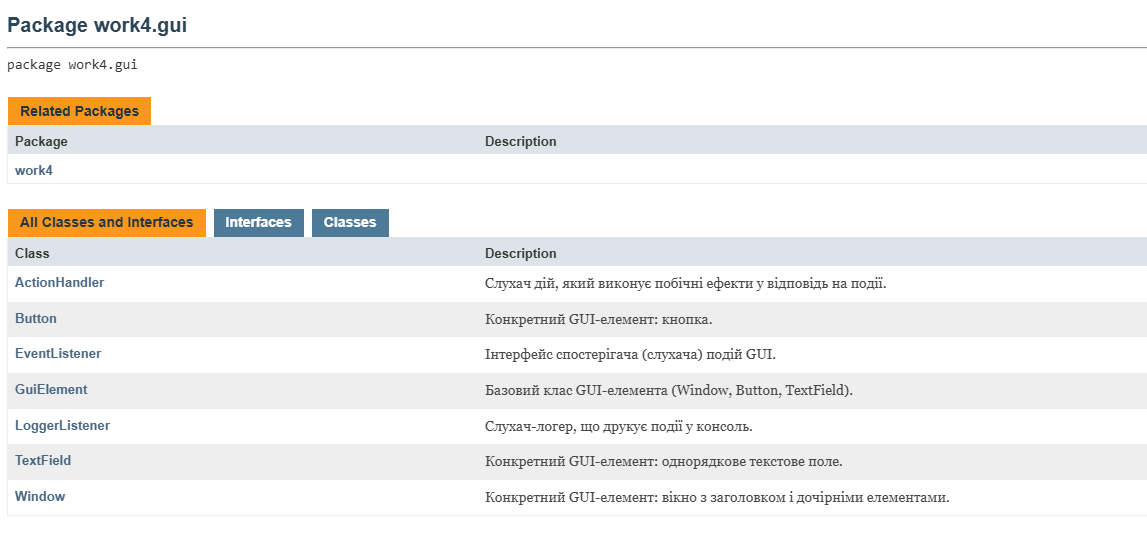
\includegraphics[width=\linewidth]{1-5.png}
        \end{subfigure}
    \end{figure}

    Щодо коду: вихідний код буде разом зі звітом, щоб не ускладнювати звіт.

    \begin{center} \textbf{\Large Практична частина (Завдання №2)} \end{center}

    Мій номер залікової книги: $4106$, звідси $4106 \text{ mod } 7 = 4$. Тому умова до 2 завдання буде:

    Необхідно розробити класи, які моделюють систему обробки запитів на технічну підтримку. Запити мають різний рівень складності, і кожен рівень обробляється відповідним співробітником:
    \begin{itemize}
    \item \textbf{Оператор підтримки} — обробляє запити \textbf{першого рівня} (простий рівень).
    \item \textbf{Інженер підтримки} — обробляє запити \textbf{другого рівня} (середній рівень).
    \item \textbf{Старший інженер підтримки} — обробляє запити \textbf{третього рівня} (складний рівень).
    \end{itemize}
    Якщо співробітник не може обробити запит, він передає його \textit{наступному в ланцюжку}, поки запит не буде оброблено.

    \paragraph{Вимоги.}
    \textbf{Інтерфейс \texttt{Handler} (Співробітник підтримки):}
    \begin{itemize}
    \item метод для обробки запиту: \verb|void handleRequest(SupportRequest request);|
    \item метод для встановлення наступного обробника в ланцюжку: \verb|void setNextHandler(Handler nextHandler);|
    \end{itemize}

    \textbf{Клас \texttt{SupportRequest} (Запит на підтримку):}
    \begin{itemize}
    \item \verb|String description| — опис запиту;
    \item \verb|int level| — рівень складності запиту (\(1\) — простий, \(2\) — середній, \(3\) — складний).
    \end{itemize}

    \textbf{Конкретні обробники запитів:}
    \begin{itemize}
    \item \texttt{OperatorSupport} — обробляє запити першого рівня;
    \item \texttt{EngineerSupport} — обробляє запити другого рівня;
    \item \texttt{SeniorEngineerSupport} — обробляє запити третього рівня.
    \end{itemize}
    Кожен обробник перевіряє рівень запиту; якщо він не відповідає компетенції, передає запит наступному обробнику.

    \textbf{Забезпечення слабкої зв'язності:}
    \begin{itemize}
    \item клас запиту не знає, хто його обробляє;
    \item клас обробника не знає, хто буде наступним у ланцюжку, окрім того, що він передасть запит далі.
    \end{itemize}

    \textbf{У методі \texttt{main} продемонструвати:}
    \begin{itemize}
    \item побудову ланцюжка обробників: \emph{оператор} \(\to\) \emph{інженер} \(\to\) \emph{старший інженер};
    \item обробку кількох запитів різного рівня складності;
    \item ситуацію, коли поточний обробник не може опрацювати запит і передає його далі по ланцюжку до успішної обробки.
    \end{itemize}

    \textbf{\underline{Загальна структура проекту до компіляції:}}

    \begin{minted}{text}
PS C:\Users\artem\Desktop\reps\university_roadmap\semestr3\software engineering\labs\lab4\additional> tree /f /a
Folder PATH listing
Volume serial number is 1A5B-F8AF
C:.
|   build.xml
|
\---src
    \---work4
        \---chain
                AbstractSupportHandler.java
                DemoChain.java
                EngineerSupport.java
                Handler.java
                OperatorSupport.java
                SeniorEngineerSupport.java
                SupportRequest.java
    \end{minted}

    \textbf{\underline{Перевірка:}}

    \begin{minted}{text}
PS C:\Users\artem\Desktop\reps\university_roadmap\semestr3\software engineering\labs\lab4\additional> ant -p 
Buildfile: C:\Users\artem\Desktop\reps\university_roadmap\semestr3\software engineering\labs\lab4\additional\build.xml

Main targets:

 clean    Remove all generated files
 compile  Compile Java sources
 dist     Perform full build (clean, compile, jar, javadoc)
 help     Show available build tasks
 jar      Package into an executable JAR file
 javadoc  Generate API documentation (Javadoc)
 run      Run the main class
Default target: dist
    \end{minted}

    \textbf{\underline{Загальна структура проекту після компіляції:}}

    \begin{minted}{text}
PS C:\Users\artem\Desktop\reps\university_roadmap\semestr3\software engineering\labs\lab4\additional> ant
Buildfile: C:\Users\artem\Desktop\reps\university_roadmap\semestr3\software engineering\labs\lab4\additional\build.xml

clean:

init:
    [mkdir] Created dir: C:\Users\artem\Desktop\reps\university_roadmap\semestr3\software engineering\labs\lab4\additional\build\classes
    [mkdir] Created dir: C:\Users\artem\Desktop\reps\university_roadmap\semestr3\software engineering\labs\lab4\additional\dist
    [mkdir] Created dir: C:\Users\artem\Desktop\reps\university_roadmap\semestr3\software engineering\labs\lab4\additional\docs

compile:
    [javac] Compiling 7 source files to C:\Users\artem\Desktop\reps\university_roadmap\semestr3\software engineering\labs\lab4\additional\build\classes
     [echo] Compilation completed successfully.

jar:
      [jar] Building jar: C:\Users\artem\Desktop\reps\university_roadmap\semestr3\software engineering\labs\lab4\additional\dist\work4-chain-demo.jar
     [echo] JAR file created: dist/work4-chain-demo.jar

javadoc:
  [javadoc] Generating Javadoc
  [javadoc] Javadoc execution
  [javadoc] Loading source files for package work4.chain...
  [javadoc] Constructing Javadoc information...
  [javadoc] Building index for all the packages and classes...
  [javadoc] Standard Doclet version 21.0.9+7-LTS-338
  [javadoc] Building tree for all the packages and classes...
  [javadoc] C:\Users\artem\Desktop\reps\university_roadmap\semestr3\software engineering\labs\lab4\additional\src\work4\chain\AbstractSupportHandler.java:6: error: unknown tag: pattern
  [javadoc]  * @pattern Chain of Responsibility: Concrete Handler (base)
  [javadoc]    ^
  [javadoc] C:\Users\artem\Desktop\reps\university_roadmap\semestr3\software engineering\labs\lab4\additional\src\work4\chain\Handler.java:5: error: unknown tag: pattern
  [javadoc]  * @pattern Chain of Responsibility: Handler
  [javadoc]    ^
  [javadoc] Generating C:\Users\artem\Desktop\reps\university_roadmap\semestr3\software engineering\labs\lab4\additional\docs\work4\chain\AbstractSupportHandler.html...
  [javadoc] C:\Users\artem\Desktop\reps\university_roadmap\semestr3\software engineering\labs\lab4\additional\src\work4\chain\AbstractSupportHandler.java:8: warning: use of default constructor, which does not provide a comment
  [javadoc] public abstract class AbstractSupportHandler implements Handler {
  [javadoc]                 ^
  [javadoc] Generating C:\Users\artem\Desktop\reps\university_roadmap\semestr3\software engineering\labs\lab4\additional\docs\work4\chain\DemoChain.html...
  [javadoc] C:\Users\artem\Desktop\reps\university_roadmap\semestr3\software engineering\labs\lab4\additional\src\work4\chain\DemoChain.java:7: warning: use of default constructor, which does not provide a comment
  [javadoc] public class DemoChain {
  [javadoc]        ^
  [javadoc] C:\Users\artem\Desktop\reps\university_roadmap\semestr3\software engineering\labs\lab4\additional\src\work4\chain\DemoChain.java:8: warning: no comment
  [javadoc]     public static void main(String[] args) {
  [javadoc]                        ^
  [javadoc] Generating C:\Users\artem\Desktop\reps\university_roadmap\semestr3\software engineering\labs\lab4\additional\docs\work4\chain\EngineerSupport.html...
  [javadoc] C:\Users\artem\Desktop\reps\university_roadmap\semestr3\software engineering\labs\lab4\additional\src\work4\chain\EngineerSupport.java:6: warning: use of default constructor, which does not provide a comment
  [javadoc] public final class EngineerSupport extends AbstractSupportHandler {
  [javadoc]              ^
  [javadoc] Generating C:\Users\artem\Desktop\reps\university_roadmap\semestr3\software engineering\labs\lab4\additional\docs\work4\chain\Handler.html...
  [javadoc] Generating C:\Users\artem\Desktop\reps\university_roadmap\semestr3\software engineering\labs\lab4\additional\docs\work4\chain\OperatorSupport.html...
  [javadoc] C:\Users\artem\Desktop\reps\university_roadmap\semestr3\software engineering\labs\lab4\additional\src\work4\chain\OperatorSupport.java:6: warning: use of default constructor, which does not provide a comment
  [javadoc] public final class OperatorSupport extends AbstractSupportHandler {
  [javadoc]              ^
  [javadoc] Generating C:\Users\artem\Desktop\reps\university_roadmap\semestr3\software engineering\labs\lab4\additional\docs\work4\chain\SeniorEngineerSupport.html...
  [javadoc] C:\Users\artem\Desktop\reps\university_roadmap\semestr3\software engineering\labs\lab4\additional\src\work4\chain\SeniorEngineerSupport.java:6: warning: use of default constructor, which does not provide a comment
  [javadoc] public final class SeniorEngineerSupport extends AbstractSupportHandler {
  [javadoc]              ^
  [javadoc] Generating C:\Users\artem\Desktop\reps\university_roadmap\semestr3\software engineering\labs\lab4\additional\docs\work4\chain\SupportRequest.html...
  [javadoc] C:\Users\artem\Desktop\reps\university_roadmap\semestr3\software engineering\labs\lab4\additional\src\work4\chain\SupportRequest.java:15: warning: no main description
  [javadoc]      * @param description ???? ??????
  [javadoc]        ^
  [javadoc] C:\Users\artem\Desktop\reps\university_roadmap\semestr3\software engineering\labs\lab4\additional\src\work4\chain\SupportRequest.java:23: warning: no main description
  [javadoc]     /** @return ???? ?????? */
  [javadoc]         ^
  [javadoc] C:\Users\artem\Desktop\reps\university_roadmap\semestr3\software engineering\labs\lab4\additional\src\work4\chain\SupportRequest.java:26: warning: no main description
  [javadoc]     /** @return ?????? ?????????? (1..3) */
  [javadoc]         ^
  [javadoc] Generating C:\Users\artem\Desktop\reps\university_roadmap\semestr3\software engineering\labs\lab4\additional\docs\work4\chain\package-summary.html...
  [javadoc] Generating C:\Users\artem\Desktop\reps\university_roadmap\semestr3\software engineering\labs\lab4\additional\docs\work4\chain\package-tree.html...
  [javadoc] Generating C:\Users\artem\Desktop\reps\university_roadmap\semestr3\software engineering\labs\lab4\additional\docs\work4\chain\class-use\AbstractSupportHandler.html...
  [javadoc] Generating C:\Users\artem\Desktop\reps\university_roadmap\semestr3\software engineering\labs\lab4\additional\docs\work4\chain\class-use\DemoChain.html...
  [javadoc] Generating C:\Users\artem\Desktop\reps\university_roadmap\semestr3\software engineering\labs\lab4\additional\docs\work4\chain\class-use\EngineerSupport.html...
  [javadoc] Generating C:\Users\artem\Desktop\reps\university_roadmap\semestr3\software engineering\labs\lab4\additional\docs\work4\chain\class-use\Handler.html...
  [javadoc] Generating C:\Users\artem\Desktop\reps\university_roadmap\semestr3\software engineering\labs\lab4\additional\docs\work4\chain\class-use\OperatorSupport.html...
  [javadoc] Generating C:\Users\artem\Desktop\reps\university_roadmap\semestr3\software engineering\labs\lab4\additional\docs\work4\chain\class-use\SeniorEngineerSupport.html...
  [javadoc] Generating C:\Users\artem\Desktop\reps\university_roadmap\semestr3\software engineering\labs\lab4\additional\docs\work4\chain\class-use\SupportRequest.html...
  [javadoc] Generating C:\Users\artem\Desktop\reps\university_roadmap\semestr3\software engineering\labs\lab4\additional\docs\work4\chain\package-use.html...
  [javadoc] Generating C:\Users\artem\Desktop\reps\university_roadmap\semestr3\software engineering\labs\lab4\additional\docs\overview-tree.html...
  [javadoc] Building index for all classes...
  [javadoc] Generating C:\Users\artem\Desktop\reps\university_roadmap\semestr3\software engineering\labs\lab4\additional\docs\allclasses-index.html...
  [javadoc] Generating C:\Users\artem\Desktop\reps\university_roadmap\semestr3\software engineering\labs\lab4\additional\docs\allpackages-index.html...
  [javadoc] Generating C:\Users\artem\Desktop\reps\university_roadmap\semestr3\software engineering\labs\lab4\additional\docs\index-files\index-1.html...
  [javadoc] Generating C:\Users\artem\Desktop\reps\university_roadmap\semestr3\software engineering\labs\lab4\additional\docs\index-files\index-2.html...
  [javadoc] Generating C:\Users\artem\Desktop\reps\university_roadmap\semestr3\software engineering\labs\lab4\additional\docs\index-files\index-3.html...
  [javadoc] Generating C:\Users\artem\Desktop\reps\university_roadmap\semestr3\software engineering\labs\lab4\additional\docs\index-files\index-4.html...
  [javadoc] Generating C:\Users\artem\Desktop\reps\university_roadmap\semestr3\software engineering\labs\lab4\additional\docs\index-files\index-5.html...
  [javadoc] Generating C:\Users\artem\Desktop\reps\university_roadmap\semestr3\software engineering\labs\lab4\additional\docs\index-files\index-6.html...
  [javadoc] Generating C:\Users\artem\Desktop\reps\university_roadmap\semestr3\software engineering\labs\lab4\additional\docs\index-files\index-7.html...
  [javadoc] Generating C:\Users\artem\Desktop\reps\university_roadmap\semestr3\software engineering\labs\lab4\additional\docs\index-files\index-8.html...
  [javadoc] Generating C:\Users\artem\Desktop\reps\university_roadmap\semestr3\software engineering\labs\lab4\additional\docs\index-files\index-9.html...
  [javadoc] Generating C:\Users\artem\Desktop\reps\university_roadmap\semestr3\software engineering\labs\lab4\additional\docs\index-files\index-10.html...
  [javadoc] Generating C:\Users\artem\Desktop\reps\university_roadmap\semestr3\software engineering\labs\lab4\additional\docs\index-files\index-11.html...
  [javadoc] Generating C:\Users\artem\Desktop\reps\university_roadmap\semestr3\software engineering\labs\lab4\additional\docs\search.html...
  [javadoc] Generating C:\Users\artem\Desktop\reps\university_roadmap\semestr3\software engineering\labs\lab4\additional\docs\index.html...
  [javadoc] Generating C:\Users\artem\Desktop\reps\university_roadmap\semestr3\software engineering\labs\lab4\additional\docs\help-doc.html...
  [javadoc] 2 errors
  [javadoc] 9 warnings
     [echo] Javadoc generated in: docs

dist:
     [echo] Distribution build completed successfully.

BUILD SUCCESSFUL
Total time: 2 seconds

    PS C:\Users\artem\Desktop\reps\university_roadmap\semestr3\software engineering\labs\lab4\additional> tree /f /a
Folder PATH listing
Volume serial number is 1A5B-F8AF
C:.
|   build.xml
|   
+---build
|   \---classes
|       \---work4
|           \---chain
|                   AbstractSupportHandler.class
|                   DemoChain.class
|                   EngineerSupport.class
|                   Handler.class
|                   OperatorSupport.class
|                   SeniorEngineerSupport.class
|                   SupportRequest.class
|
+---dist
|       work4-chain-demo.jar
|
+---docs
|   |   allclasses-index.html
|   |   allpackages-index.html
|   |   copy.svg
|   |   element-list
|   |   help-doc.html
|   |   index.html
|   |   link.svg
|   |   member-search-index.js
|   |   module-search-index.js
|   |   overview-tree.html
|   |   package-search-index.js
|   |   script.js
|   |   search-page.js
|   |   search.html
|   |   search.js
|   |   stylesheet.css
|   |   tag-search-index.js
|   |   type-search-index.js
|   |
|   +---index-files
|   |       index-1.html
|   |       index-10.html
|   |       index-11.html
|   |       index-2.html
|   |       index-3.html
|   |       index-4.html
|   |       index-5.html
|   |       index-6.html
|   |       index-7.html
|   |       index-8.html
|   |       index-9.html
|   |
|   +---legal
|   |       COPYRIGHT
|   |       jquery.md
|   |       jqueryUI.md
|   |       LICENSE
|   |
|   +---resources
|   |       glass.png
|   |       x.png
|   |
|   +---script-dir
|   |       jquery-3.7.1.min.js
|   |       jquery-ui.min.css
|   |       jquery-ui.min.js
|   |
|   \---work4
|       \---chain
|           |   AbstractSupportHandler.html
|           |   DemoChain.html
|           |   EngineerSupport.html
|           |   Handler.html
|           |   OperatorSupport.html
|           |   package-summary.html
|           |   package-tree.html
|           |   package-use.html
|           |   SeniorEngineerSupport.html
|           |   SupportRequest.html
|           |
|           \---class-use
|                   AbstractSupportHandler.html
|                   DemoChain.html
|                   EngineerSupport.html
|                   Handler.html
|                   OperatorSupport.html
|                   SeniorEngineerSupport.html
|                   SupportRequest.html
|
\---src
    \---work4
        \---chain
                AbstractSupportHandler.java
                DemoChain.java
                EngineerSupport.java
                Handler.java
                OperatorSupport.java
                SeniorEngineerSupport.java
                SupportRequest.java
    \end{minted}

    \textbf{\underline{Результат виконання (демонстрації програми):}}

    \begin{minted}{text}
PS C:\Users\artem\Desktop\reps\university_roadmap\semestr3\software engineering\labs\lab4\additional> ant run 
Buildfile: C:\Users\artem\Desktop\reps\university_roadmap\semestr3\software engineering\labs\lab4\additional\build.xml

init:

compile:
     [echo] Compilation completed successfully.

run:
     [java] OperatorSupport: handled (L1) -> SupportRequest{level=1, desc="Password reset"}
     [java] OperatorSupport -> passing to EngineerSupport for SupportRequest{level=2, desc="VPN not connecting"}
     [java] EngineerSupport: handled (L2) -> SupportRequest{level=2, desc="VPN not connecting"}
     [java] OperatorSupport -> passing to EngineerSupport for SupportRequest{level=3, desc="Production outage"}
     [java] EngineerSupport -> passing to SeniorEngineerSupport for SupportRequest{level=3, desc="Production outage"}
     [java] SeniorEngineerSupport: handled (L3) -> SupportRequest{level=3, desc="Production outage"}
     [java] OperatorSupport -> passing to EngineerSupport for SupportRequest{level=99, desc="Exotic issue"}
     [java] EngineerSupport -> passing to SeniorEngineerSupport for SupportRequest{level=99, desc="Exotic issue"}
     [java] SeniorEngineerSupport -> no next handler, request dropped: SupportRequest{level=99, desc="Exotic issue"}

BUILD SUCCESSFUL
Total time: 0 seconds
    \end{minted}

    \newpage

    \textbf{\underline{Скріншот наявності документації:}}

    \begin{figure}[h!]
        \centering

        \begin{subfigure}{1.0\textwidth}
            \centering
            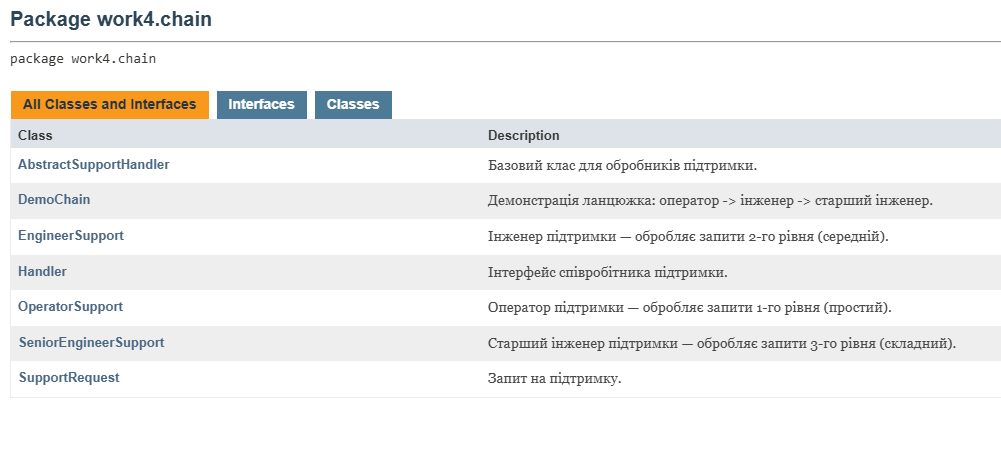
\includegraphics[width=\linewidth]{2-1.png}
        \end{subfigure}\vfill
        \begin{subfigure}{1.0\textwidth}
            \centering
            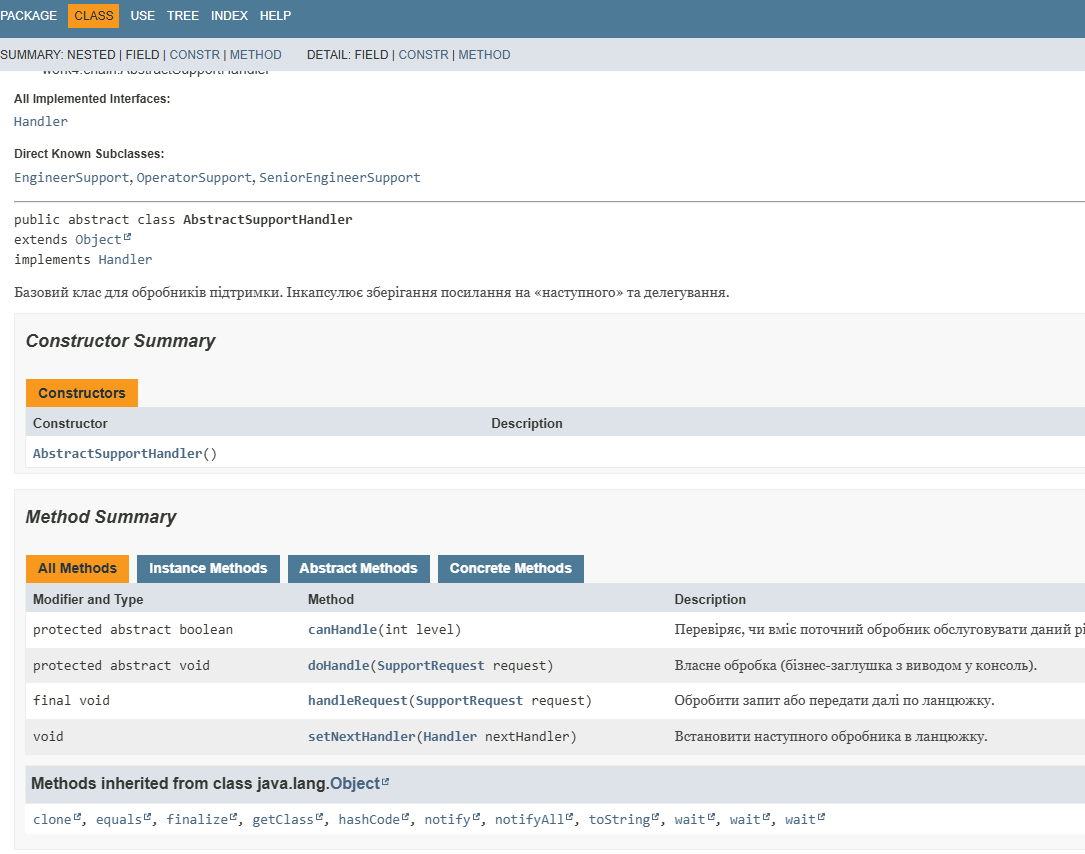
\includegraphics[width=\linewidth]{2-2.png}
        \end{subfigure}
    \end{figure}

    Код до цього також вирішив не вставляти у звіт. Вихідний код буде наданий разом зі звітом.

    \newpage

    \textbf{\underline{Висновок:}} 
    У результаті виконання лабораторної роботи було розроблено два програмні проєкти, що реалізують поведінкові шаблони проєктування — \textbf{Observer} та \textbf{Chain of Responsibility}.

    \setlength{\parindent}{1.5em}

    \subsection*{1. Шаблон \textbf{Observer} (Спостерігач)}
    Було змодельовано спрощену систему графічного інтерфейсу користувача (GUI), до складу якої входять класи \texttt{GuiElement}, \texttt{Button}, \texttt{TextField}, \texttt{Window}, а також інтерфейс \texttt{EventListener}.  
    GUI-елементи виступають як джерела подій, а слухачі — як об’єкти-спостерігачі, що реагують на зміни стану або дії користувача.  
    Було реалізовано механізм підписки та сповіщення про події (\texttt{addListener()}, \texttt{removeListener()}, \texttt{notifyListeners()}).  
    У демонстраційній програмі (\texttt{DemoGuiSwing}) показано роботу системи: натискання кнопки, зміна тексту та закриття вікна автоматично викликають відповідні реакції слухачів.  
    Завдяки шаблону \textbf{Observer} забезпечено слабку зв’язність між елементами та гнучке розширення системи.

    \subsection*{2. Шаблон \textbf{Chain of Responsibility} (Ланцюжок обов’язків)}
    Було реалізовано систему обробки запитів на технічну підтримку, де кожен обробник відповідає за певний рівень складності запитів: \texttt{OperatorSupport} — прості, \texttt{EngineerSupport} — середні, \texttt{SeniorEngineerSupport} — складні.  
    Інтерфейс \texttt{Handler} визначає методи для обробки запиту та передачі його наступному обробнику.  
    Якщо поточний обробник не може розв’язати проблему, запит передається далі по ланцюжку до того, хто може його опрацювати.  
    У демонстраційному класі \texttt{DemoChain} продемонстровано правильну роботу механізму: кожен запит опрацьовується на відповідному рівні або відхиляється, якщо підходящий обробник відсутній.  
    Шаблон \textbf{Chain of Responsibility} дозволив реалізувати масштабовану систему з чітким розподілом відповідальності між об’єктами.

    \subsection*{Загальні результати}
    Під час виконання роботи набуті практичні навички реалізації поведінкових шаблонів проєктування, що сприяють підвищенню модульності, розширюваності та підтримуваності програмних систем.  
    Застосування шаблонів \textbf{Observer} та \textbf{Chain of Responsibility} дало змогу продемонструвати принципи об’єктно-орієнтованого проєктування: інкапсуляцію, слабку зв’язність і делегування відповідальності між об’єктами.
 
\end{document}